%\documentclass[11pt,twocolumn]{article}
\documentclass{llncs}
\bibliographystyle{unsrt}
\usepackage{graphicx}
\usepackage{url}
\usepackage{hyperref}
\usepackage{subcaption}         % include subfigure
\bibliographystyle{splncs03}
\usepackage{color} % color selection

\begin{document}

\title{Early evaluation of the hybrid cluster with torus interconnect aimed at cost-effective molecular-dynamics simulations}

\author{%
Vladimir~V.~Stegailov\inst{1},
Alexander~Agarkov\inst{2},
Sergey~Biryukov\inst{2},
Timur~Ismagilov\inst{2},
Nikolai~Kondratyuk\inst{1}\inst{3}\inst{4},
Evgeny~Kushtanov\inst{2},
Dmitry~Makagon\inst{2},
Anatoly~Mukosey\inst{2},
Alexander~Semenov\inst{2},
Alexey~Simonov\inst{2},
Vyacheslav~Vecher\inst{1}\inst{3}
}
%
\authorrunning{V.~Stegailov et al.} % abbreviated author list (for running head)
%
\institute{Joint Institute for High Temperatures of RAS, Moscow, Russia\\
\and NICEVT, Moscow, Russia\\
\and Moscow Institute of Physics and Technology, Dolgoprudny, Russia\\
\and National Research University Higher School of Economics, Moscow, Russia
\email{v.stegailov@hse.ru}
}

\maketitle

\begin{abstract}
In this paper, we describe the Desmos cluster that consists of 32 hybrid nodes connected by a low-latency high-bandwidth Angara torus interconnect. This cluster is aimed at cost-effective classical molecular dynamics calculations. We present strong scaling benchmarks for GROMACS and compare the results with other HPC systems. \colorbox{yellow}{I suggest to remove the next sentence}. \colorbox{yellow}{I think it is our internal ''kitchen''}, \colorbox{yellow}{otherwise european scientists will think that we have Napoleon's plans :)}. Moreover, the cluster serves as a test bed for the Angara interconnect and verifies its ability to unite large MPP systems speeding-up effectively MPI-based applications. The interconnect is based on the Angara NIC that supports 3D and 4D torus network topologies. We describe the interconnect presenting typical MPI benchmarks.  
\end{abstract}


\section{Introduction}


\section{Related work}

\subsection{Scalability of classical MD on supercomputers}

A lot of work on redesigning software for HPC with GPUs and testing new hardware is done by this moment. MD codes are also become rewritten for running on CPU+coprocessor machines which allow to investigate real size and timescales in MD models. Authors of~\cite{Sun2012} show how to double the performance of running MD biomolecular model in NAMD~\cite{NAMD} with GPUs on Jaguar Cray XK6 machine with Gemini interconnect. In~\cite{Bernaschi2015} it is described how to to achieve an excellent efficiency using cluster with GPUs by using suitable memory access patterns and mechanisms like CUDA streams and profiling tools. The errors propagation in GPU systems is studied in~\cite{Li2016}.

The Mont-Blanc project is aimed to developing of the supercomputer based on ARM cores~\cite{Rajovic2016}. The main advantages of this project are flexibility in designing an application-specific system-on-chip, in turn providing the possibility in balancing performance, energy-efficiency, and cost.

The topology of connections between supercomputer nodes also influences on the scaling of the current simulation. The comparison of torus and fat tree topologies is done in~\cite{Corsetti2014} based on SIESTA electronic structure code~\cite{SIESTA} for \textit{ab initio} MD on six large-scale supercomputers. Torus topologies are showed to demonstrate a better scalability to large system sizes than those implementing fat tree topologies. Torus topology is implemented in 512-node Anton~2 MD supercomputer which allows to achieve simulation rates of multiple microseconds of physical time per day for systems with millions of atoms~\cite{Shaw2014}.

High MD code optimization for concrete supercomputer can provide better large-scaling performance than use of wide spread MD packages such as NAMD~\cite{NAMD}, GROMACS~\cite{GROMACS}, CHARMM~\cite{CHARMM}, LAMMPS and AMBER~\cite{AMBER} which can be installed almost on any machine.  In~\cite{Pennycook2013}, authors demonstrate novel code-level and algorithmic improvements to Sandia's miniMD benchmark~\cite{SandiaMD} and show that the usage of Intel Xeon Phi coprocessor provides up to 2x performance increase. The optimizations of MD code ls1mardyn are done for Intel Sandy Bridge processor including vectorization and shared-memory parallelization which allow to simulate liquid of multi-trillion Lennard-Jones particles on 146016 Cores of SuperMUC. Special MD code is developed in~\cite{Yoshii2015} called MODYLAS for machines like K-computer with torus topology. MODYLAS allows to investigate 100 ns-long MD calculation of 10 million-atom systems within 3 days (5 ms/step) by using machines as K-computer. The optimized for Intel Xeon Phi vectorization scheme is developed and applied to speed up LAMMPS calculations in~\cite{Hohnerbach2016}. The accuracy of MD with single precision is also studied.

\section{Cluster Desmos}

\begin{table}[h]
\caption{\label{tab:systems}Desmos cluster system configuration.}
\begin{center}
\renewcommand{\arraystretch}{1}
\begin{tabular}{|p{33mm}|p{80mm}|}
\hline
\textbf{Server} & Supermicro SuperServer 1018GR-T\\
\hline
\textbf{Processor} & Xeon E5-1650 v3 (6 cores, 3.0 GHz)\\
\hline
\textbf{GPU} & Nvidia GeForce GTX 1070 (1920C, 8 GB GDDR5)\\
\hline
\textbf{Memory} & DDR4 8 GB\\
\hline
\textbf{Number of nodes} & 32\\
\hline
\textbf{Interconnect} & Angara 4D-torus $4\times2\times2\times2$\\
\hline
\textbf{Operating system} & SLES 11 SP4 \\
\hline
\textbf{Compiler} & Intel Parallel Studio XE 2017 \\
\hline
\textbf{MPI} & Angara MPI (based on MPICH 3.0.4)\\
\hline
\end{tabular}
\end{center}
\end{table}

\subsection{GPU Testing}
The Nvidia GTX 1070 cards have no memory errors correction
(ECC) in contrast to the professional accelerators. For this reason
it was necessary to make sure that there is no hardware memory errors in each GPU.


Testing of each GPU was performed using MemtestG80 \cite{Haque:2010:HDS:1844765.1845231}.
Testing was performed on the available memory of the accelerator (8 GB) and wasted at least
4 hours (depending on the number of test iterations). Testing time was chosen on the basis of the results obtained in the paper \cite{Kutzner2015BestBF} and restrictions 
imposed by the number of cards and the total time of the test the entire batch. There are no errors detected during the testing process.

\subsection{Angara Interconnect}
%FIXME to dmvkt: BG, Cray, Tofu, Extoll

Angara interconnect is a Russian-designed communication network with torus topology. Inteconnect chip was developed by JSC NICEVT and manufactured by TSMC with 65 nm process. 

\begin{table}[h]
\caption{\label{tab:interconnect}Interconnects \colorbox{yellow}{FIXME! BW??}.}
\begin{center}
\renewcommand{\arraystretch}{1}
\begin{tabular}{|p{33mm}|p{20mm}|p{20mm}|p{20mm}|p{20mm}|p{20mm}|}
\hline
\textbf{Interconnect}           & BG/Q   & Cray Gemini & Tofu2    & EXTOLL & Angara \\
\hline
\textbf{Topology} 				& 5D-tor & 3D-tor      & 6D-tor ??& 3D-tor & 4D-tor\\
\hline
\textbf{Link bandwidth, Gbps}   & 16     & 75          & 100     & 100    & n/a\\
\hline
\textbf{MPI latency, ms}        & 2.5    & 1.5         & ??		 & 0.85	  & 0.85\\
\hline
\end{tabular}
\end{center}
\end{table}

In Angara architecture are used some priciples from IBM Blue Gene L/P, Cray Seastar2/Seastar2+ torus interconnects. The very similar project is EXTOLL \cite{HPCA-2015-NeuwirthFNB}.
The Angara chip supports deadlock-free adaptive routing based on bubble flow control \cite{Puente:1999:ABR:850940.852882},  direction ordered routing \cite{Adiga:2005:BGT:1665957.1665963}, \cite{Scott96thecray} and initial and final hops \cite{Scott96thecray} for fault tolerance.

Each node has a dedicated memory region available for remote access (read, write, atomic operations) from other nodes to support the OpenSHMEM and PGAS languages. Multiple parallel programming models are supported, including MPI, OpenMP, OpenSHMEM.

The network adapter is a PCI Express extension card that is connected to the adjacent nodes by up to 6 cables (or up to 8 with an extension card). The following topologies are supported: ring, 2D, 3D and 4D torus (or grid). 

\begin{figure}[h!]
\centering
   \begin{subfigure}{0.48\textwidth}
    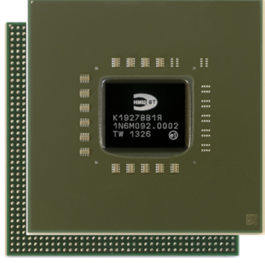
\includegraphics[width=0.8\textwidth]{img/angara_chip.png}\caption{}
   \end{subfigure}
   \begin{subfigure}{0.48\textwidth}
    \includegraphics[width=1\textwidth]{img/desmos_backpanel.jpg}\caption{}
   \end{subfigure}
\caption{(a) The ``Angara'' chip. (b) The photo of the rear side of the rack with cabling.}
\end{figure}

\section{Experimental Results}

\begin{figure}[h!]
\centering
   \begin{subfigure}{0.48\textwidth}
  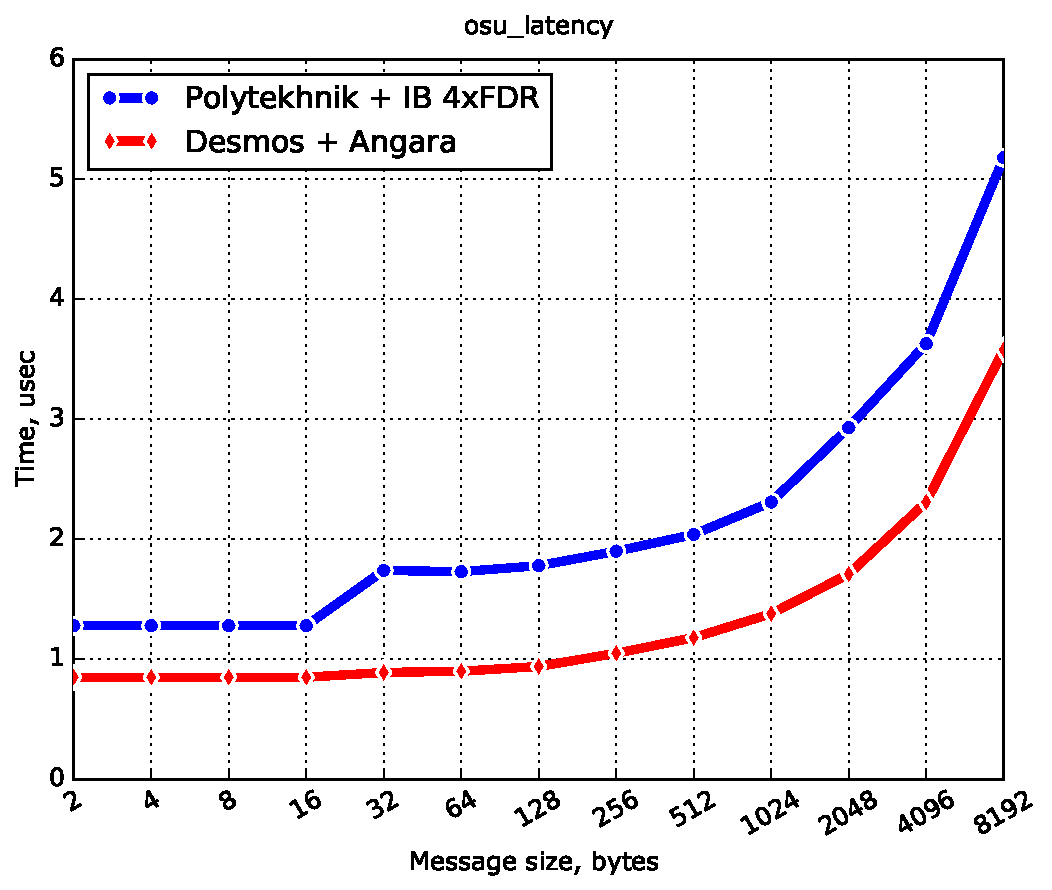
\includegraphics[width=1\textwidth]{img/osu_latency.pdf}\caption{}
  \end{subfigure}
  \begin{subfigure}{0.48\textwidth}
  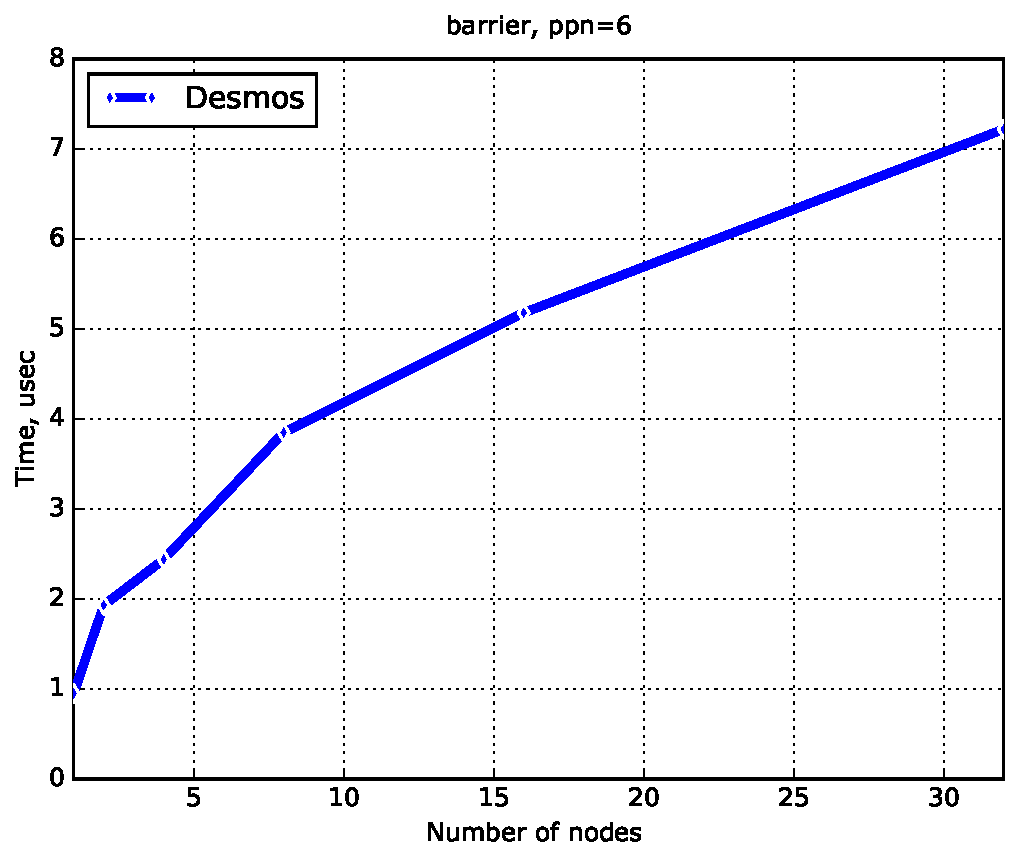
\includegraphics[width=1\textwidth]{img/barrier_ppn=6.pdf}\caption{}
   \end{subfigure}
\caption{(a) Communication latency between two adjacent Desmos nodes (OSU Micro-Benchmarks 5.3.2). (b) Intel MPI Benchmarks 2017 MPI\_Barrier, processes per node (ppn) = 6.}
\end{figure}

\begin{figure}[h!]
\centering
   \begin{subfigure}{0.48\textwidth}
  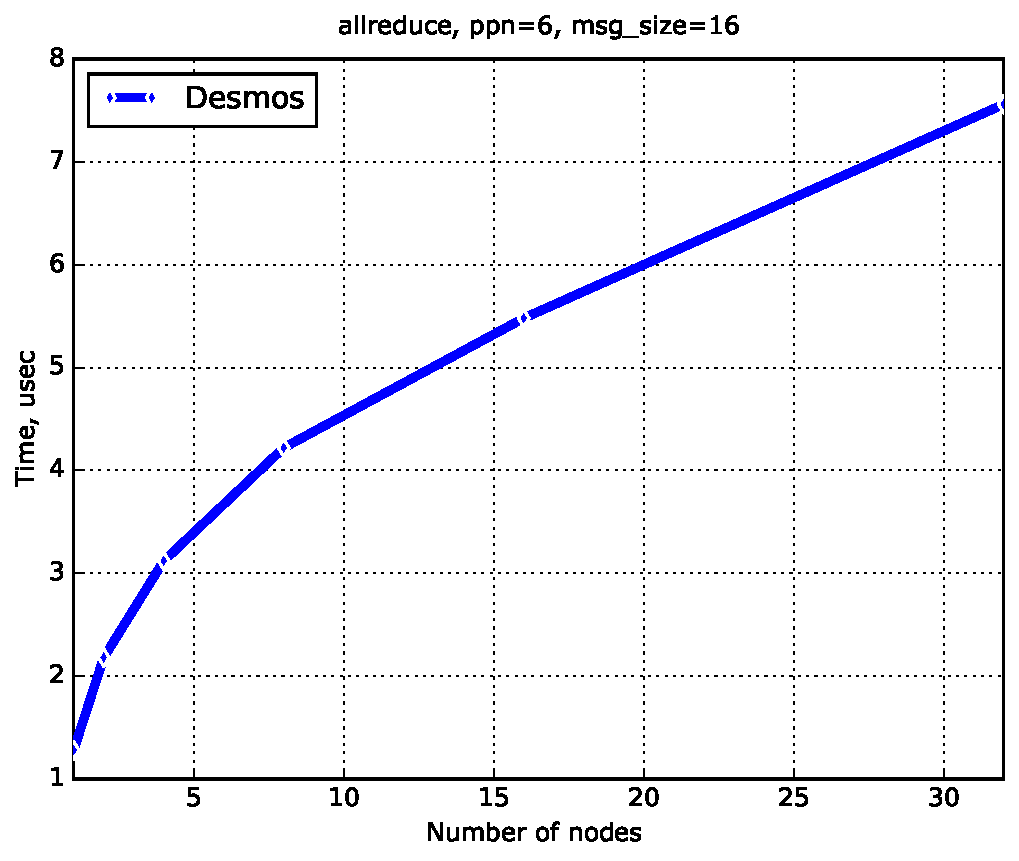
\includegraphics[width=1\textwidth]{img/allreduce_ppn=6_size=16.pdf}\caption{}
  \end{subfigure}
  \begin{subfigure}{0.48\textwidth}
  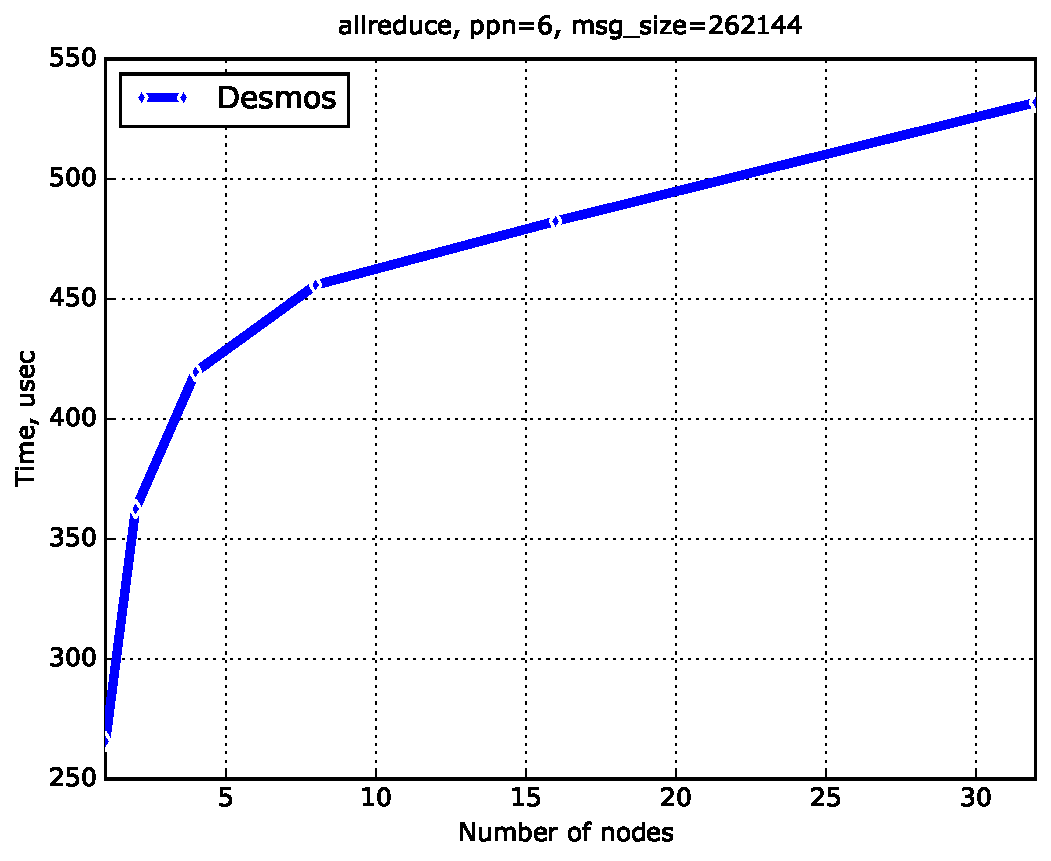
\includegraphics[width=1\textwidth]{img/allreduce_ppn=6_size=262144.pdf}\caption{}
   \end{subfigure}
\caption{FIXME: REMOVE?? Intel MPI Benchmarks 2017 MPI\_Allreduce, ppn = 6 (a) message size = 16 bytes (b) message size = 256 KB. }
\end{figure}

\newpage
\subsection{ApoA1 benchmark}

\begin{table}[h]
\caption{\label{tab:supercomputers}Info about different clusters.}
\begin{center}
\renewcommand{\arraystretch}{1}
\begin{tabular}{|p{33mm}|p{80mm}|}
\hline
\end{tabular}
\end{center}
\end{table}

The Apolipoprotein A1 in water ($\sim$100k atoms) system (ApoA1) is used to compare Desmos cluster with other supercomputers. The performances of different clusters based on ApoA1 test are shown in Fig.~\ref{ApoA1} in terms of seconds per 1 atom for 1 MD step and declared peak performance (3.236~TFlops per node consist of 6 core Xeon performance which is 0.336~TFlops and GPU performance which is estimated as 2.9~TFlops). The dotted line shows ideal scalability with performance 0.1 MFlops/atom/step.

\begin{figure}[h!]
\centering
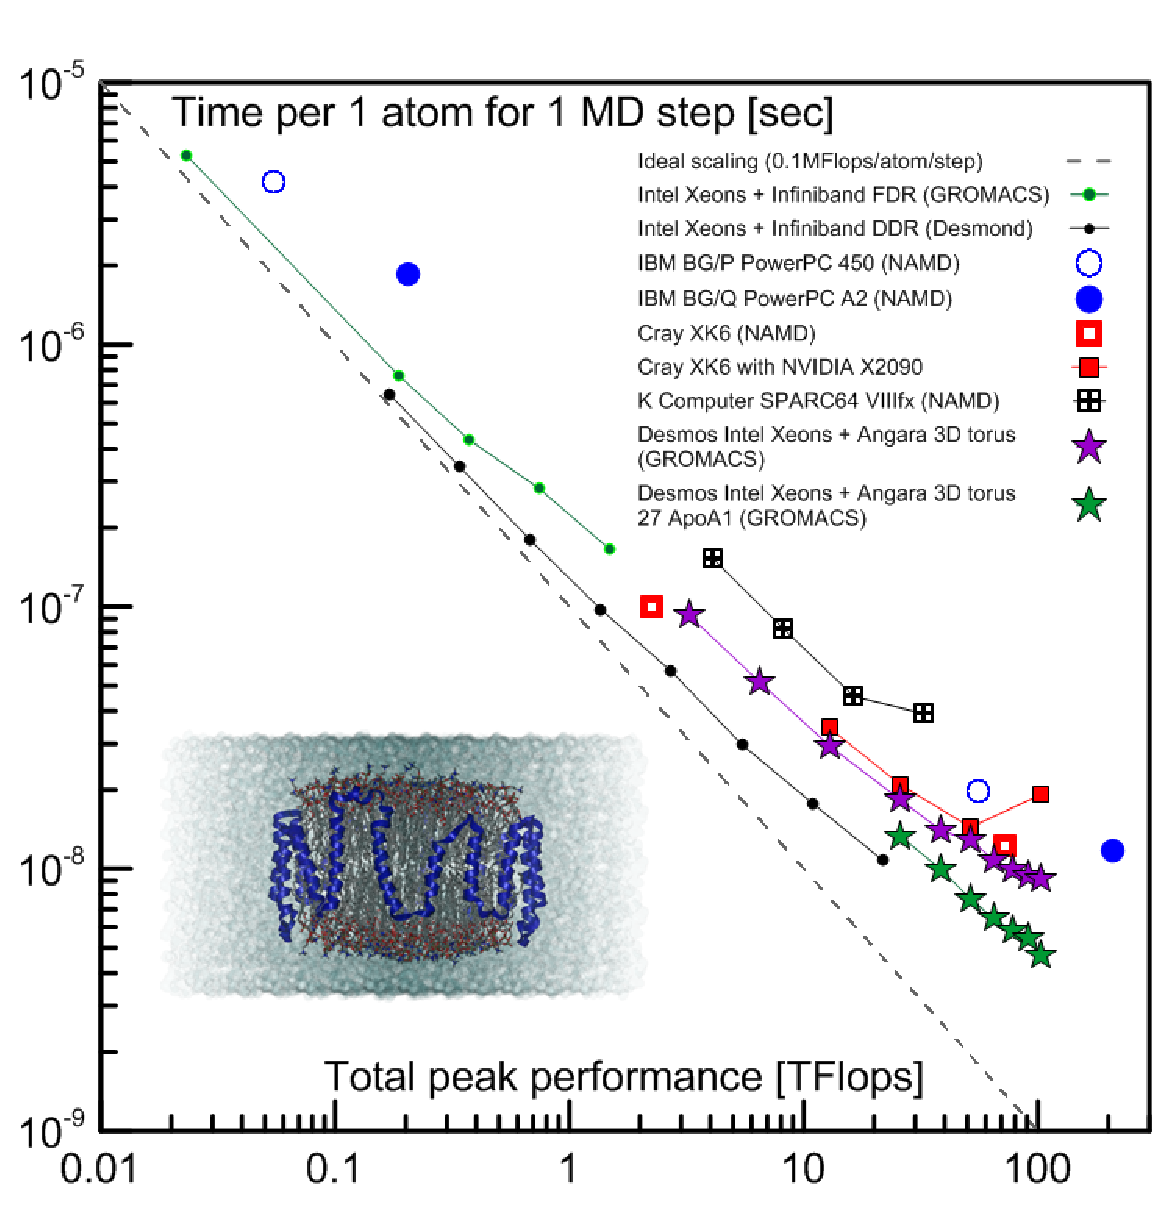
\includegraphics[width=0.8\textwidth]{img/compar_comp.eps}
\caption{\label{ApoA1}ApoA1 benchmark. Timestep per 1 atom per 1 MD step vs $R_{peak}$. The comparison of different systems.}
\end{figure}

Despite different architectures and MD software, this data can be used to analyze the applicability of some supercomputer systems for biomolecular MD system. Black and green lines with dotes show the performance of CPU cluster with Intel Xeon nodes that consist of 28 cores~\cite{Smirnov2016}. New Desmos machine (purple filled stars) with GROMACS shows better scalability then CRAY XK6 with NVIDIA X2090~\cite{Sun2012} (red filled squares) and K Computer SPARC64 Vlllfx with NAMD [?]. It also outgoes benchmarks ran on IBM BlueGene/P and BlueGene/Q~\cite{Kumar2013} (blue open and filled points correspondingly). 

Green stars are 27 times replicated ApoA1 benchmarks on Desmos machine. This result shows the continuous scaling with larger number atoms per node. It indicates the possibility for adding new nodes to Desmos without lack of performance.

\subsection{MEM and RIB benchmarks}

The work~\cite{Kutzner2015} gives a good guidelines for achieving the best performance for a minimal price in 2015. Authors compare different configurations of supercomputers using two wide spread biological benchmarks (are available at~\cite{bench}): membrane channel protein embedded in a lipid bilayer surrounded by water (MEM, $\sim $100k atoms) and ions and bacterial ribosome in water with ions (RIB, $\sim$2M atoms). GROMACS package is used for all tests. The longer simulations than in~\cite{Kutzner2015} are performed to obtain the best performance. Other benchmark options are kept the same.

\begin{figure}[h]
\centering
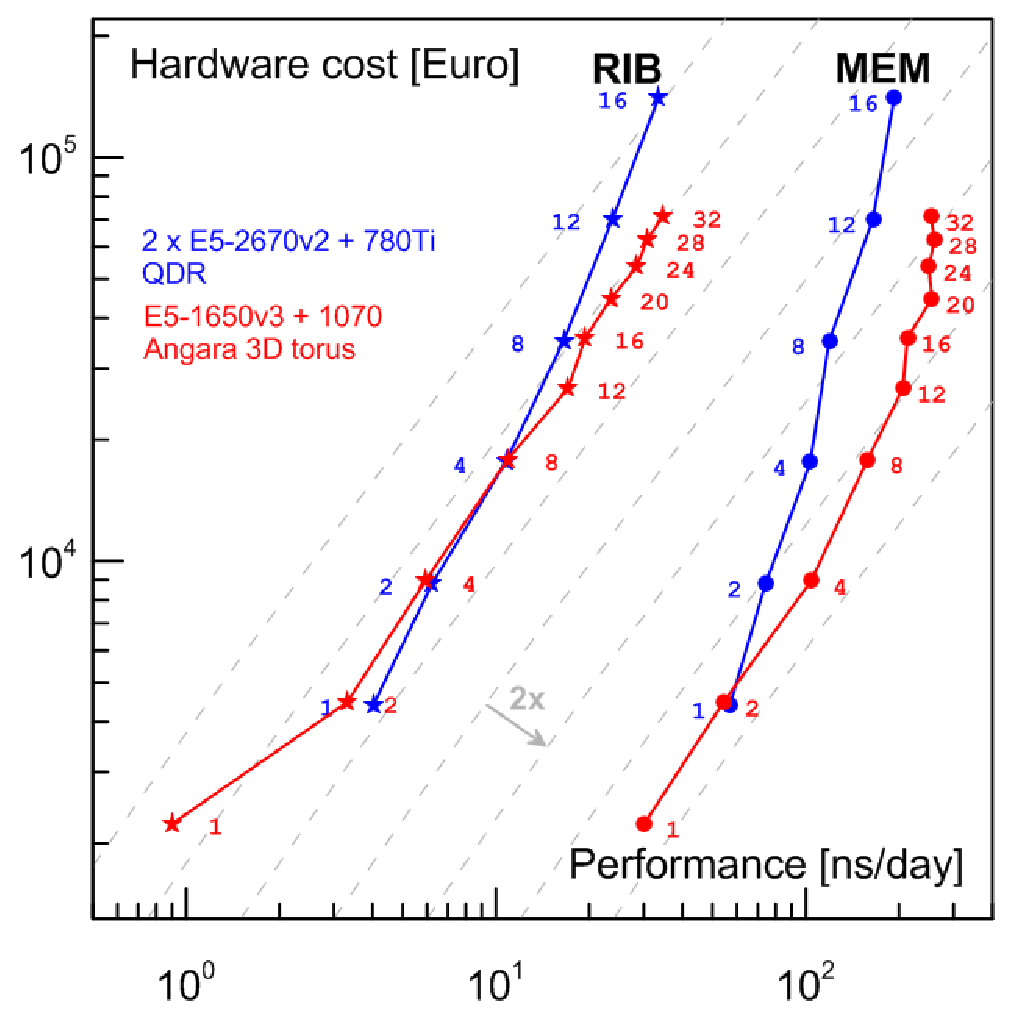
\includegraphics[width=0.8\textwidth]{img/best_bang.eps}
\caption{\label{BestBang}The cost of hardware vs achieved performance for MEM and RIB benchmarks. Dashed lines show ideal scaling. Comparison with the published results for GROMACS in~\cite{Kutzner2015}.}
\end{figure}

We compare the results obtained on Desmos cluster with the best choice of~\cite{Kutzner2015}: the nodes consist of 2 sockets Xeon E5-2670v2 with 780Ti and connected via InfiniBand QDR. The costs of hardware in euros are displayed on Y axis and the performance in ns/day is shown on X axis in Fig.~\ref{BestBang}. The numbers show the amount of nodes used. Grey lines indicate ideal scaling.

Desmos (red color) shows better weak scaling for MEM benchmark than system configuration provided by~\cite{Kutzner2015} (blue color). The saturation is achieved after 20 nodes which corresponds to the small amount of atoms per node. In the case of RIB benchmark, Desmos demonstrates ideal scaling after 16 nodes which shows that the productivity can be increased with more number of nodes.


\section{Conclusions}

The work of the JIHT team (N.K., V.S. and V.V.) was supported by the grant No.\,14-50-00124 of the Russian Science Foundation (this work includes the development of the cluster node architecture, the preliminary benchmarks, the purchase of the Desmos cluster). The NICEVT team developed the ``Angara'' interconnect and the corresponding low-level software stack, built and tuned the Desmos cluster).

\textbf{\textit{Comment for reviewers}}. Unfortunately, Angara interconnect bandwidth is the subject of non-disclosure agreement of Angara project.



\bibliography{references,references_MD}

\end{document}
